% !TeX spellcheck = en_GB


\section{Numerical Experiments}



\subsection{Pure Advection}








\subsection{PyGyro}

Our main point of comparing the Arakawa method to the Semi-Lagrangian scheme are the conserved quantities: the mass
\begin{equation}
	\int f(r, \theta, z, v_\parallel) \d r \d \theta \d z \d v_\parallel
\end{equation}
and $l^2$-norm
\begin{equation}
	\left[\int f^2(r, \theta, z, v_\parallel) \d r \d \theta \d z \d v_\parallel\right]^\frac{1}{2}
\end{equation}
of the distribution function, and the potential energy
\begin{equation}
	\int \left(f(r, \theta, z, v_\parallel) - f_\text{eq}(r, v_\parallel)\right) \Phi(r, \theta, z) \d r \d \theta \d z \d v_\parallel
\end{equation}
, as well as the not necessarily conserved kinetic energy
\begin{equation}
	\int \left(f(r, \theta, z, v_\parallel) - f_\text{eq}(r, v_\parallel)\right) v^2_\parallel \d r \d \theta \d z \d v_\parallel
\end{equation}

From a simulation with grid size $[r:128, \theta:256, z:128, v_\parallel :72]$ and time step-size $\Delta t = 1$ we plot for the above mentioned 4 quantities the absolute error (figure \ref{fig:abserr}), the relative error (figure \ref{fig:relerr}), and the relative error on a logarithmic scale (\ref{fig:relerrlog}) before and after the poloidal advection step.

We can clearly see that the Arakawa scheme preserves the conserved quantities much better than semi-Lagrangian scheme. In the linear phase, the error is of order of machine precision. Only very late in the non-linear phase becomes the relative error bigger, but is still one or two orders of magnitude smaller than in the semi-Lagrangian scheme.

The kinetic energy is also much better preserved.

The same study with time-step size $\Delta t = 2$ was done (figures \ref{fig:abserr_dt2}, \ref{fig:relerr_dt2}, \ref{fig:relerrlog_dt2}) and yields the same results. It is therefore interesting to compare the results of the poloidal advection step for the Arakawa method for the two time step-sizes; these results are shown in figures \ref{fig:abserr_akw}, \ref{fig:relerr_akw}, \ref{fig:relerrlog_akw}. We see that the doubling of the time step-size results in double the absolute error for the conserved quantities, and about a factor of 5 for the kinetic energy.

\begin{figure}
	\centering
	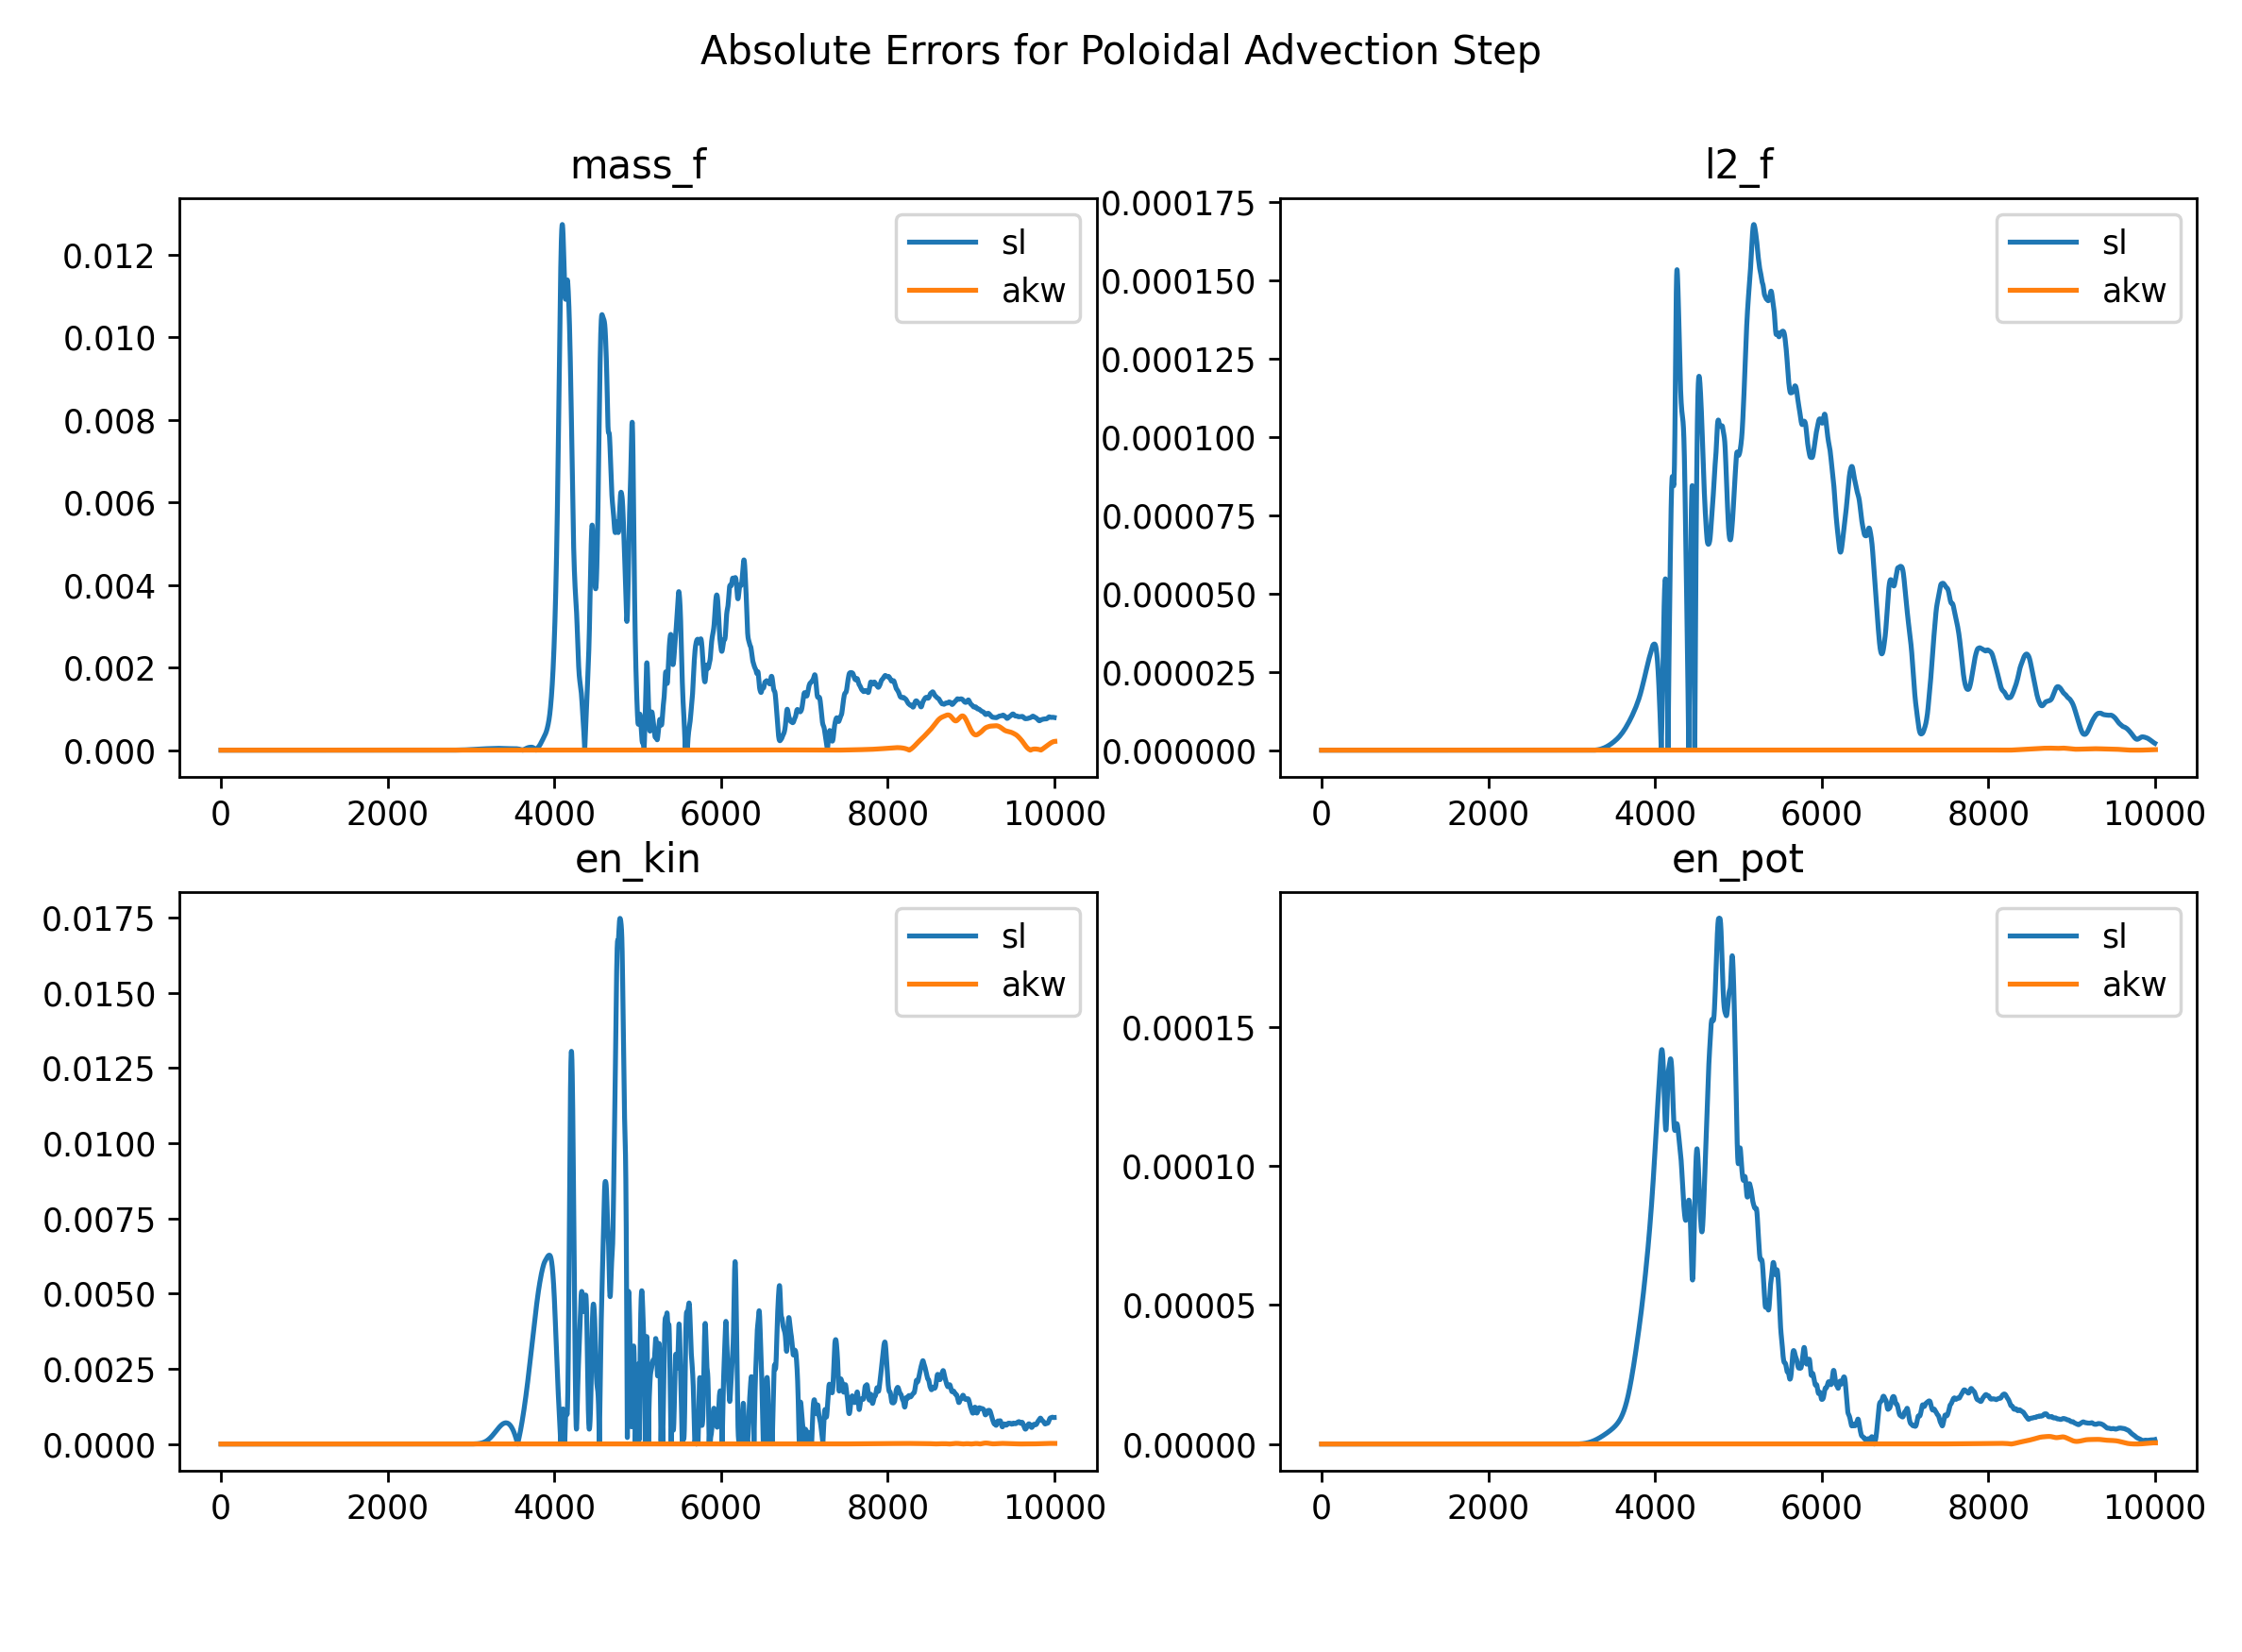
\includegraphics[width=0.9\linewidth]{abs_err}
	\caption{The absolute error for different quantities before and after the poloidal advection step.}
	\label{fig:abserr}
\end{figure}


\begin{figure}
	\centering
	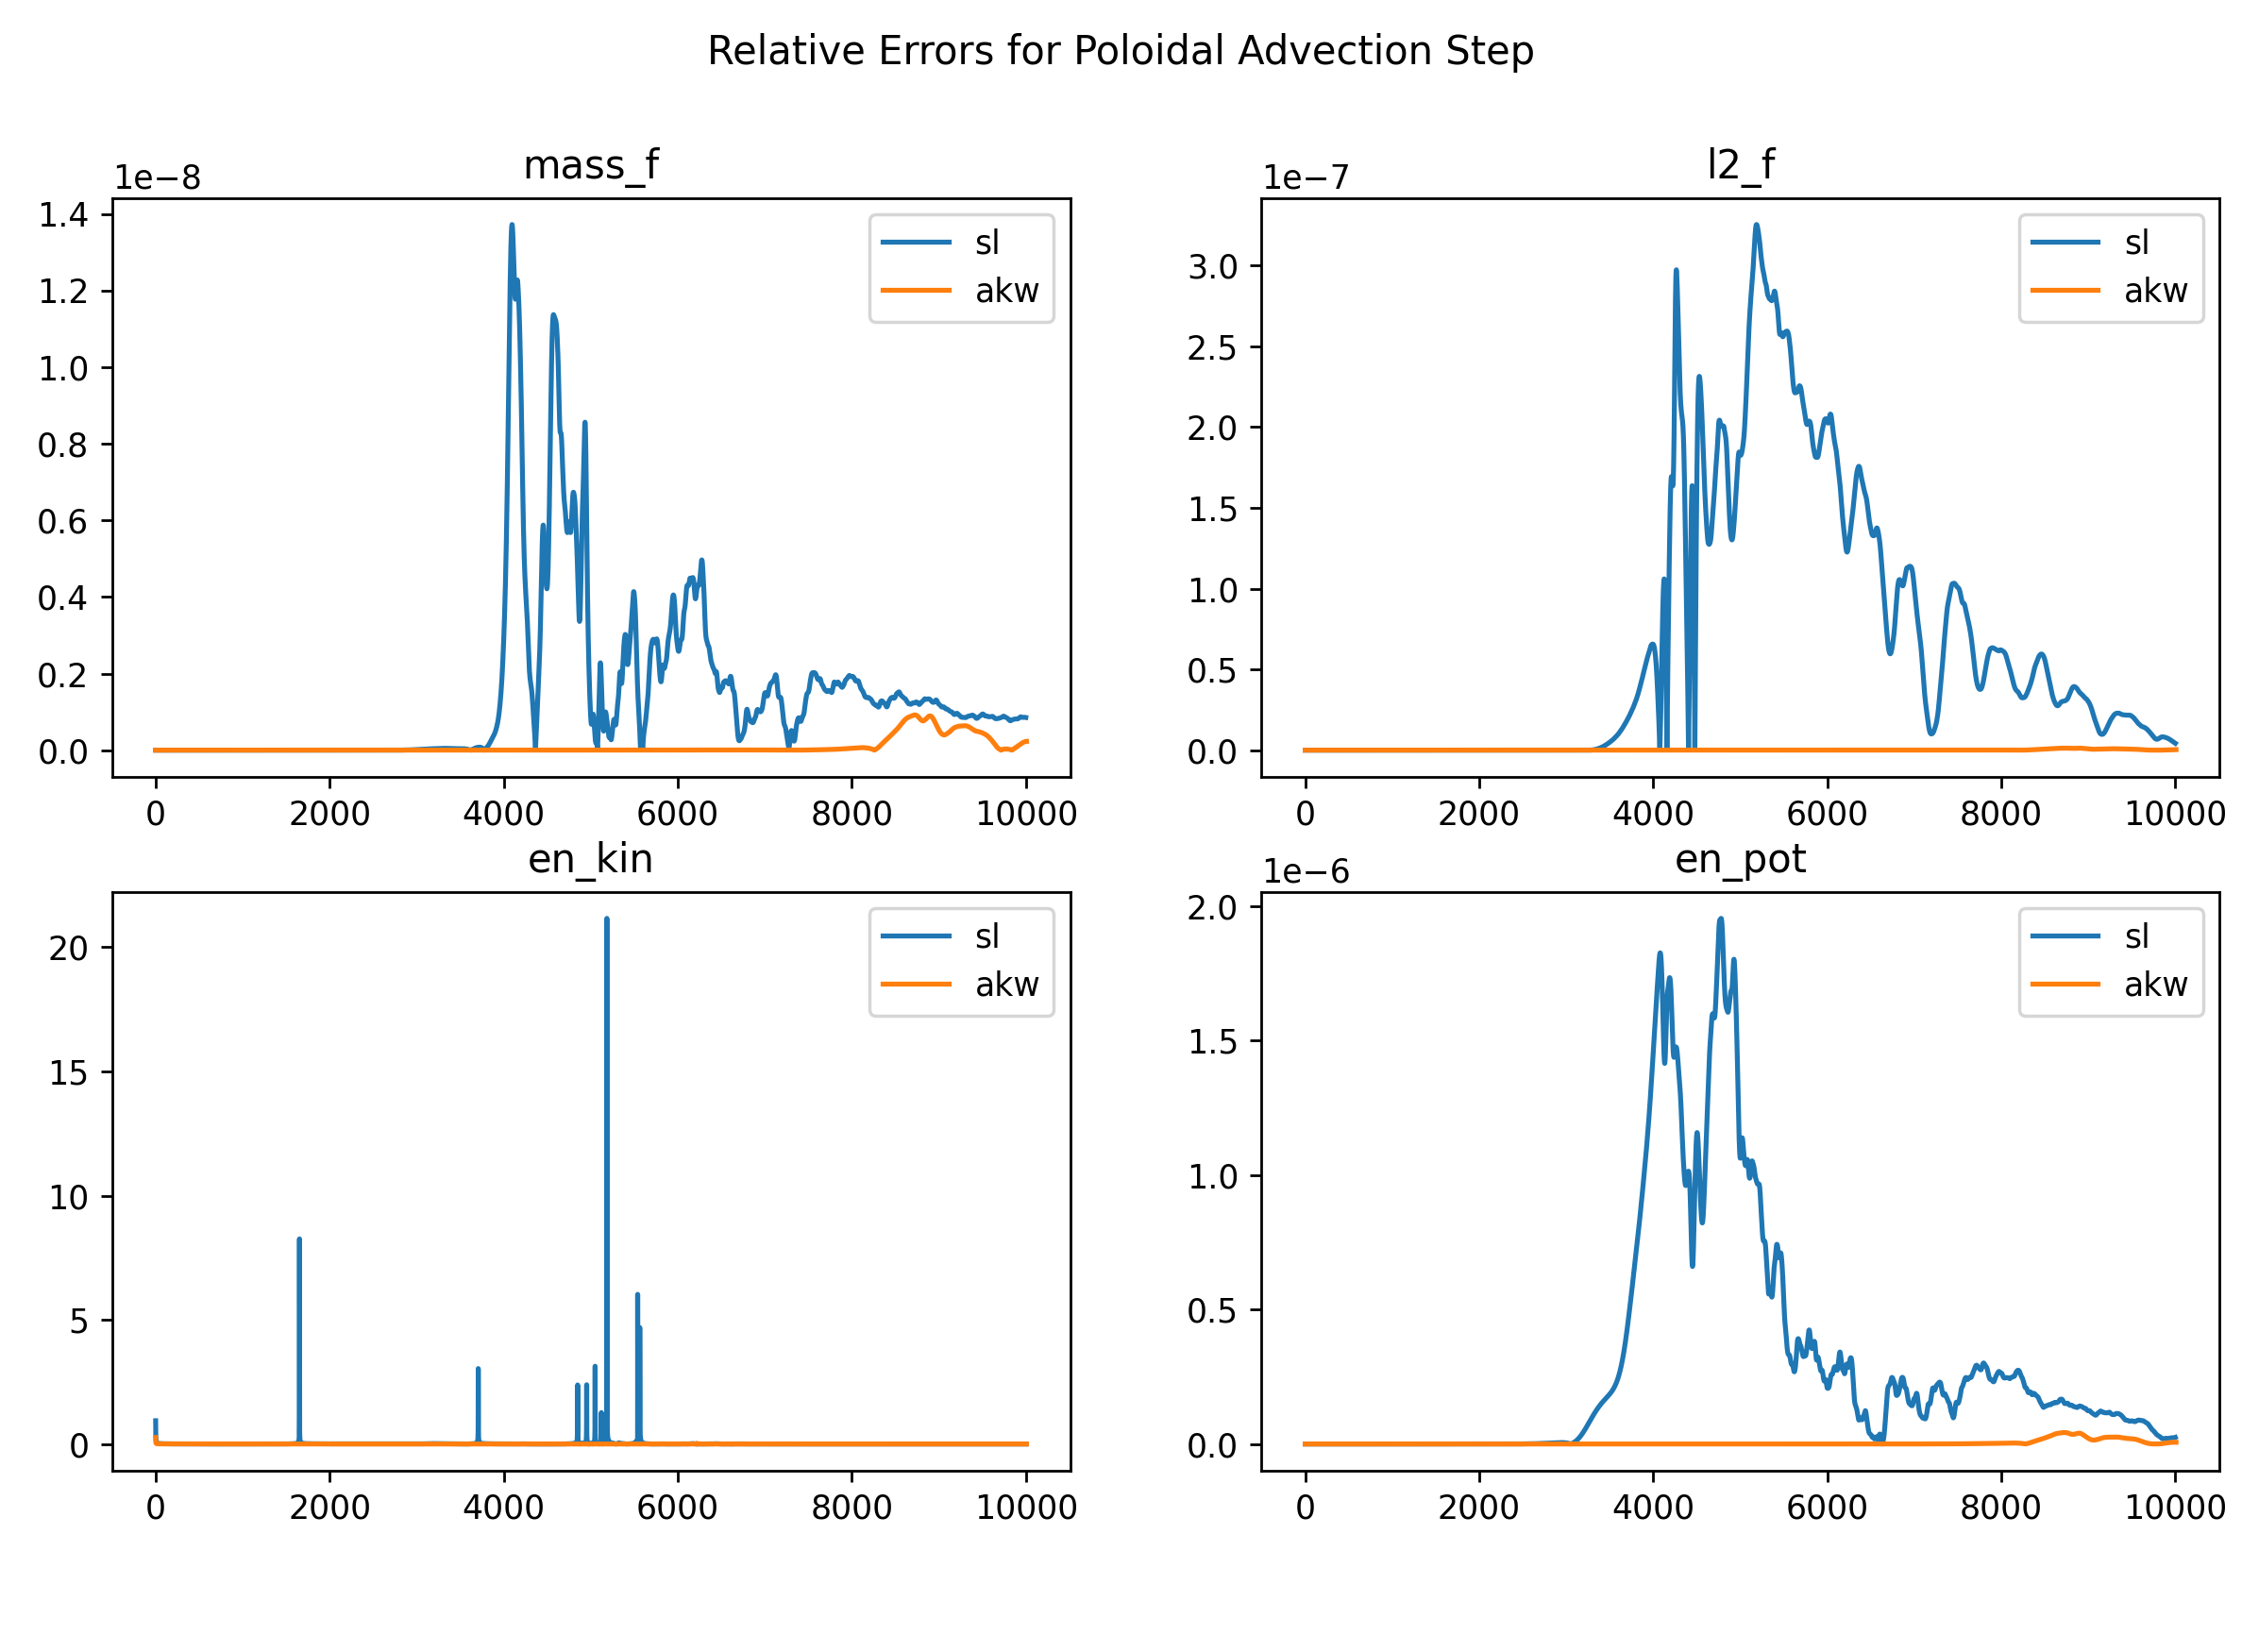
\includegraphics[width=0.9\linewidth]{rel_err}
	\caption{The relative error for different quantities before and after the poloidal advection step.}
	\label{fig:relerr}
\end{figure}


\begin{figure}
	\centering
	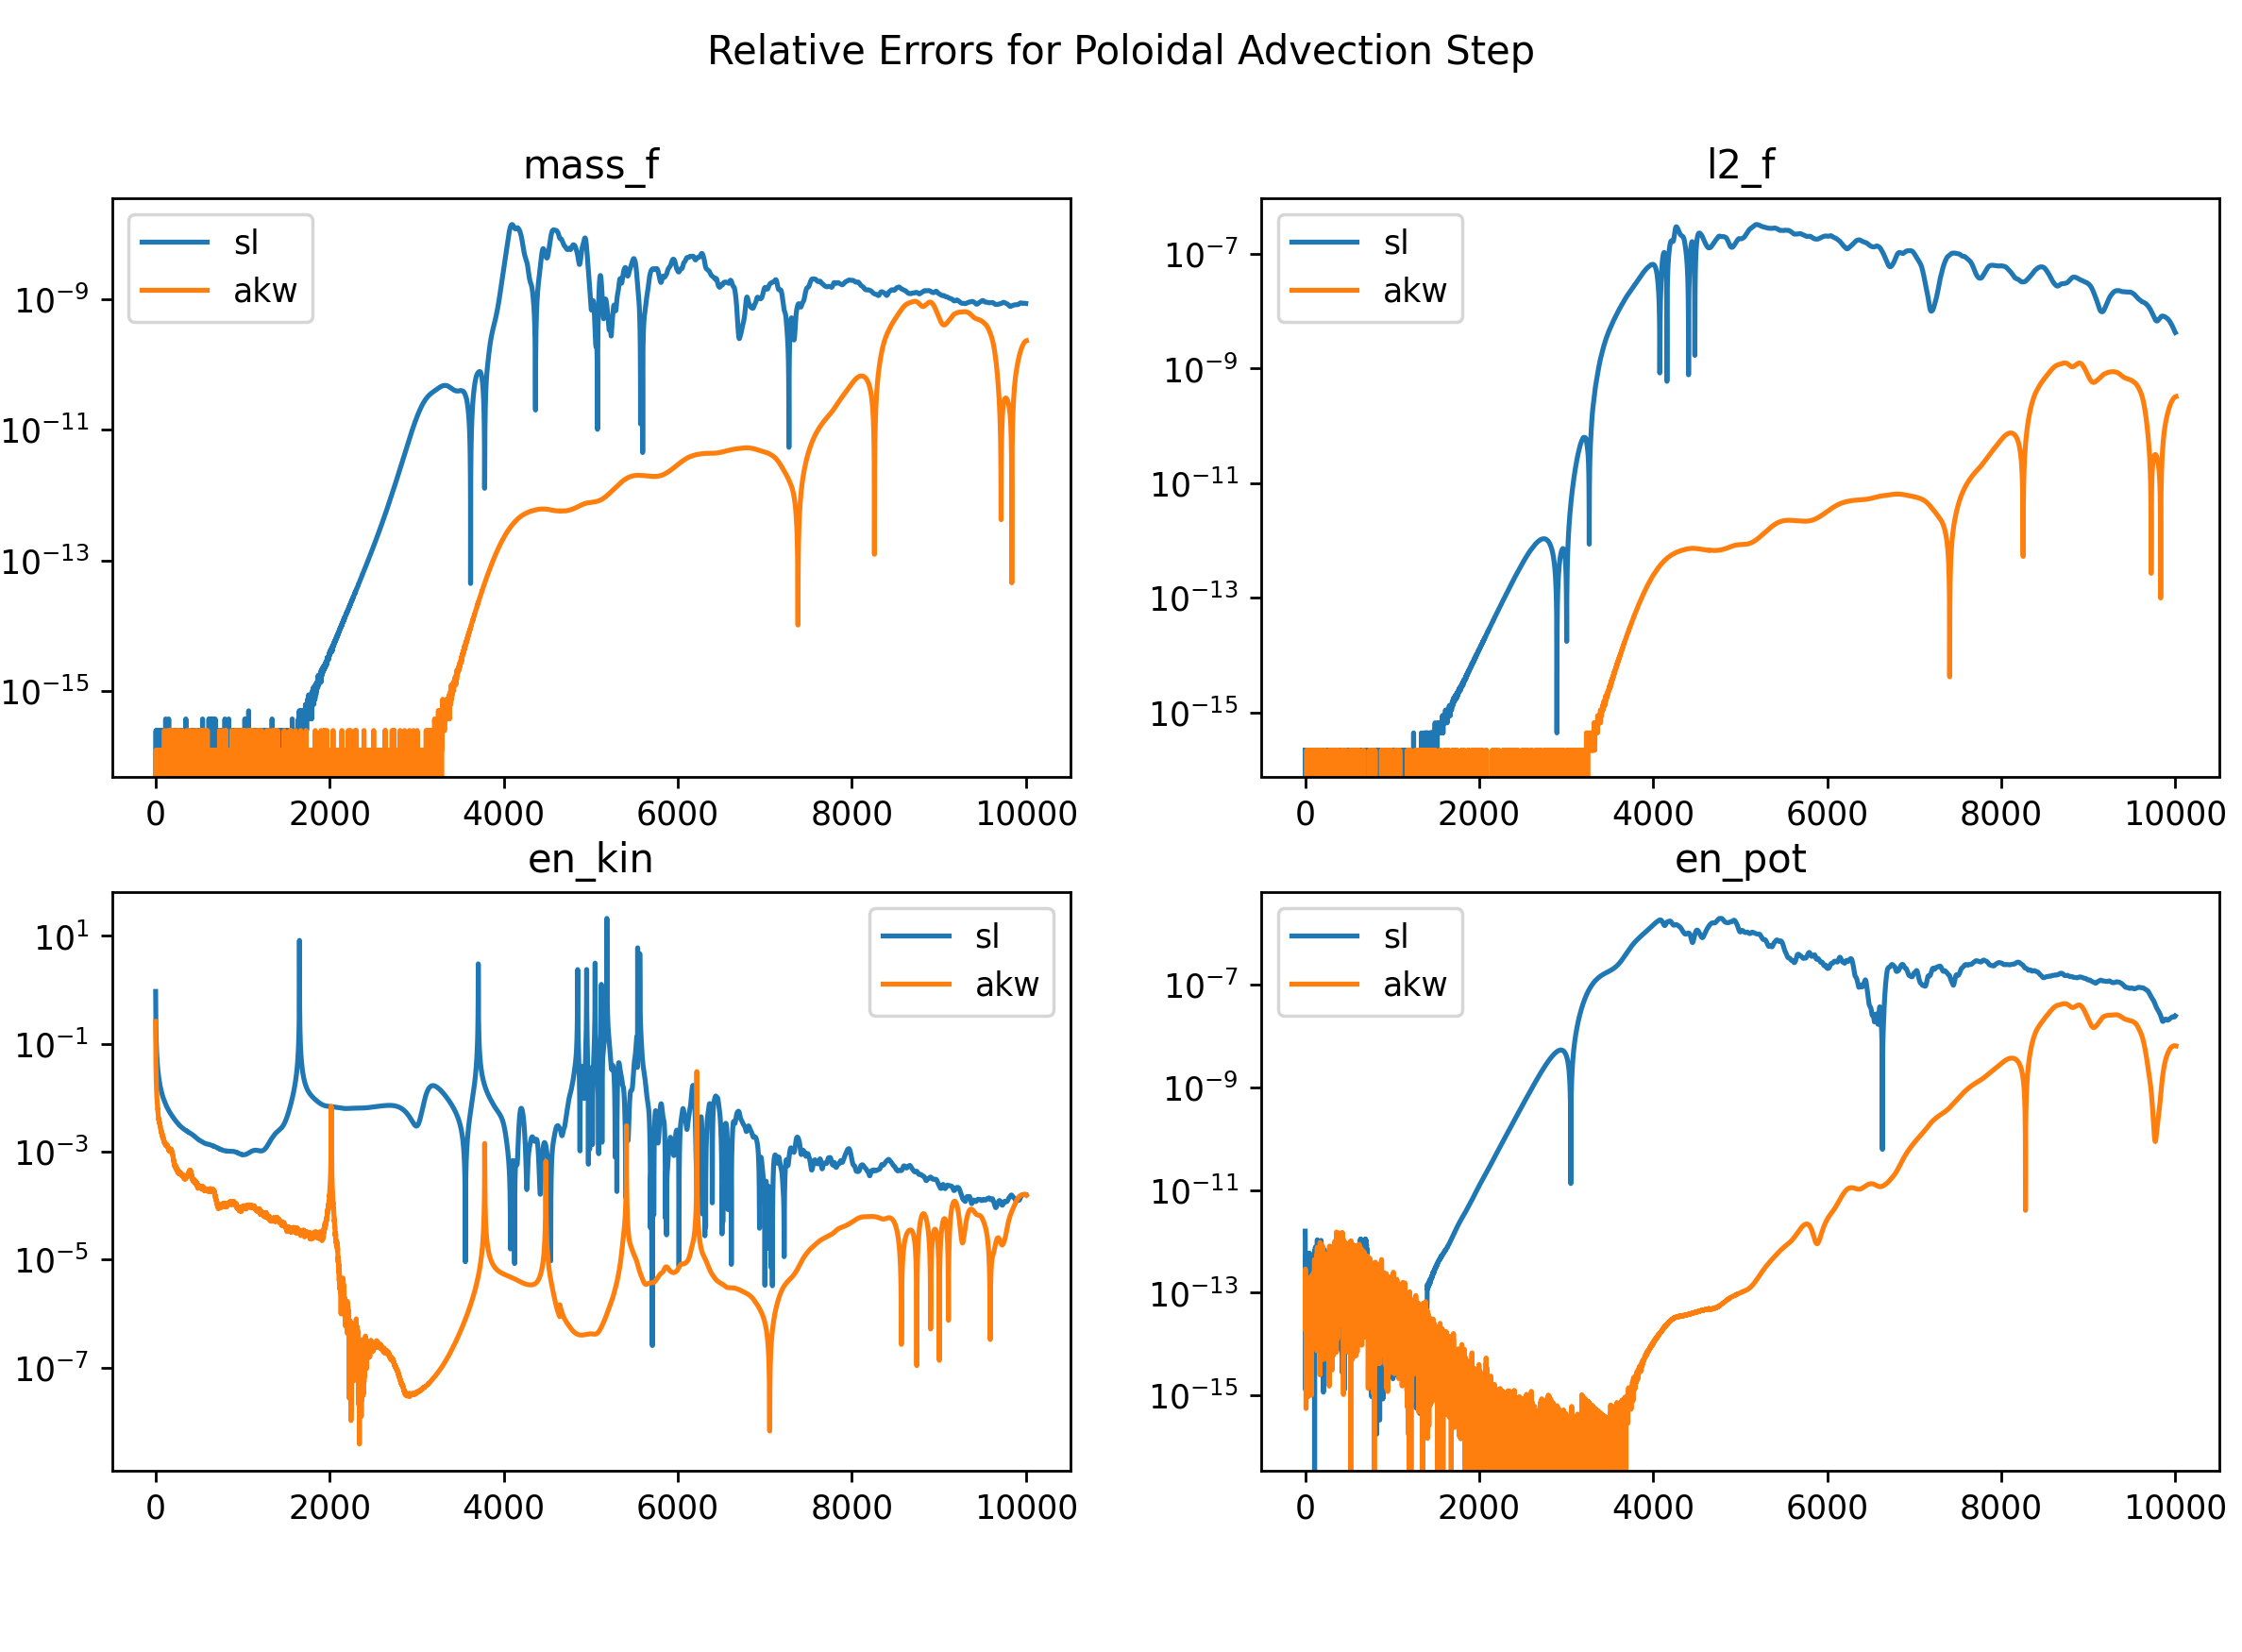
\includegraphics[width=0.9\linewidth]{rel_err_log}
	\caption{The relative error for different quantities before and after the poloidal advection step on a semi-logarithmic scale.}
	\label{fig:relerrlog}
\end{figure}


\begin{figure}
	\centering
	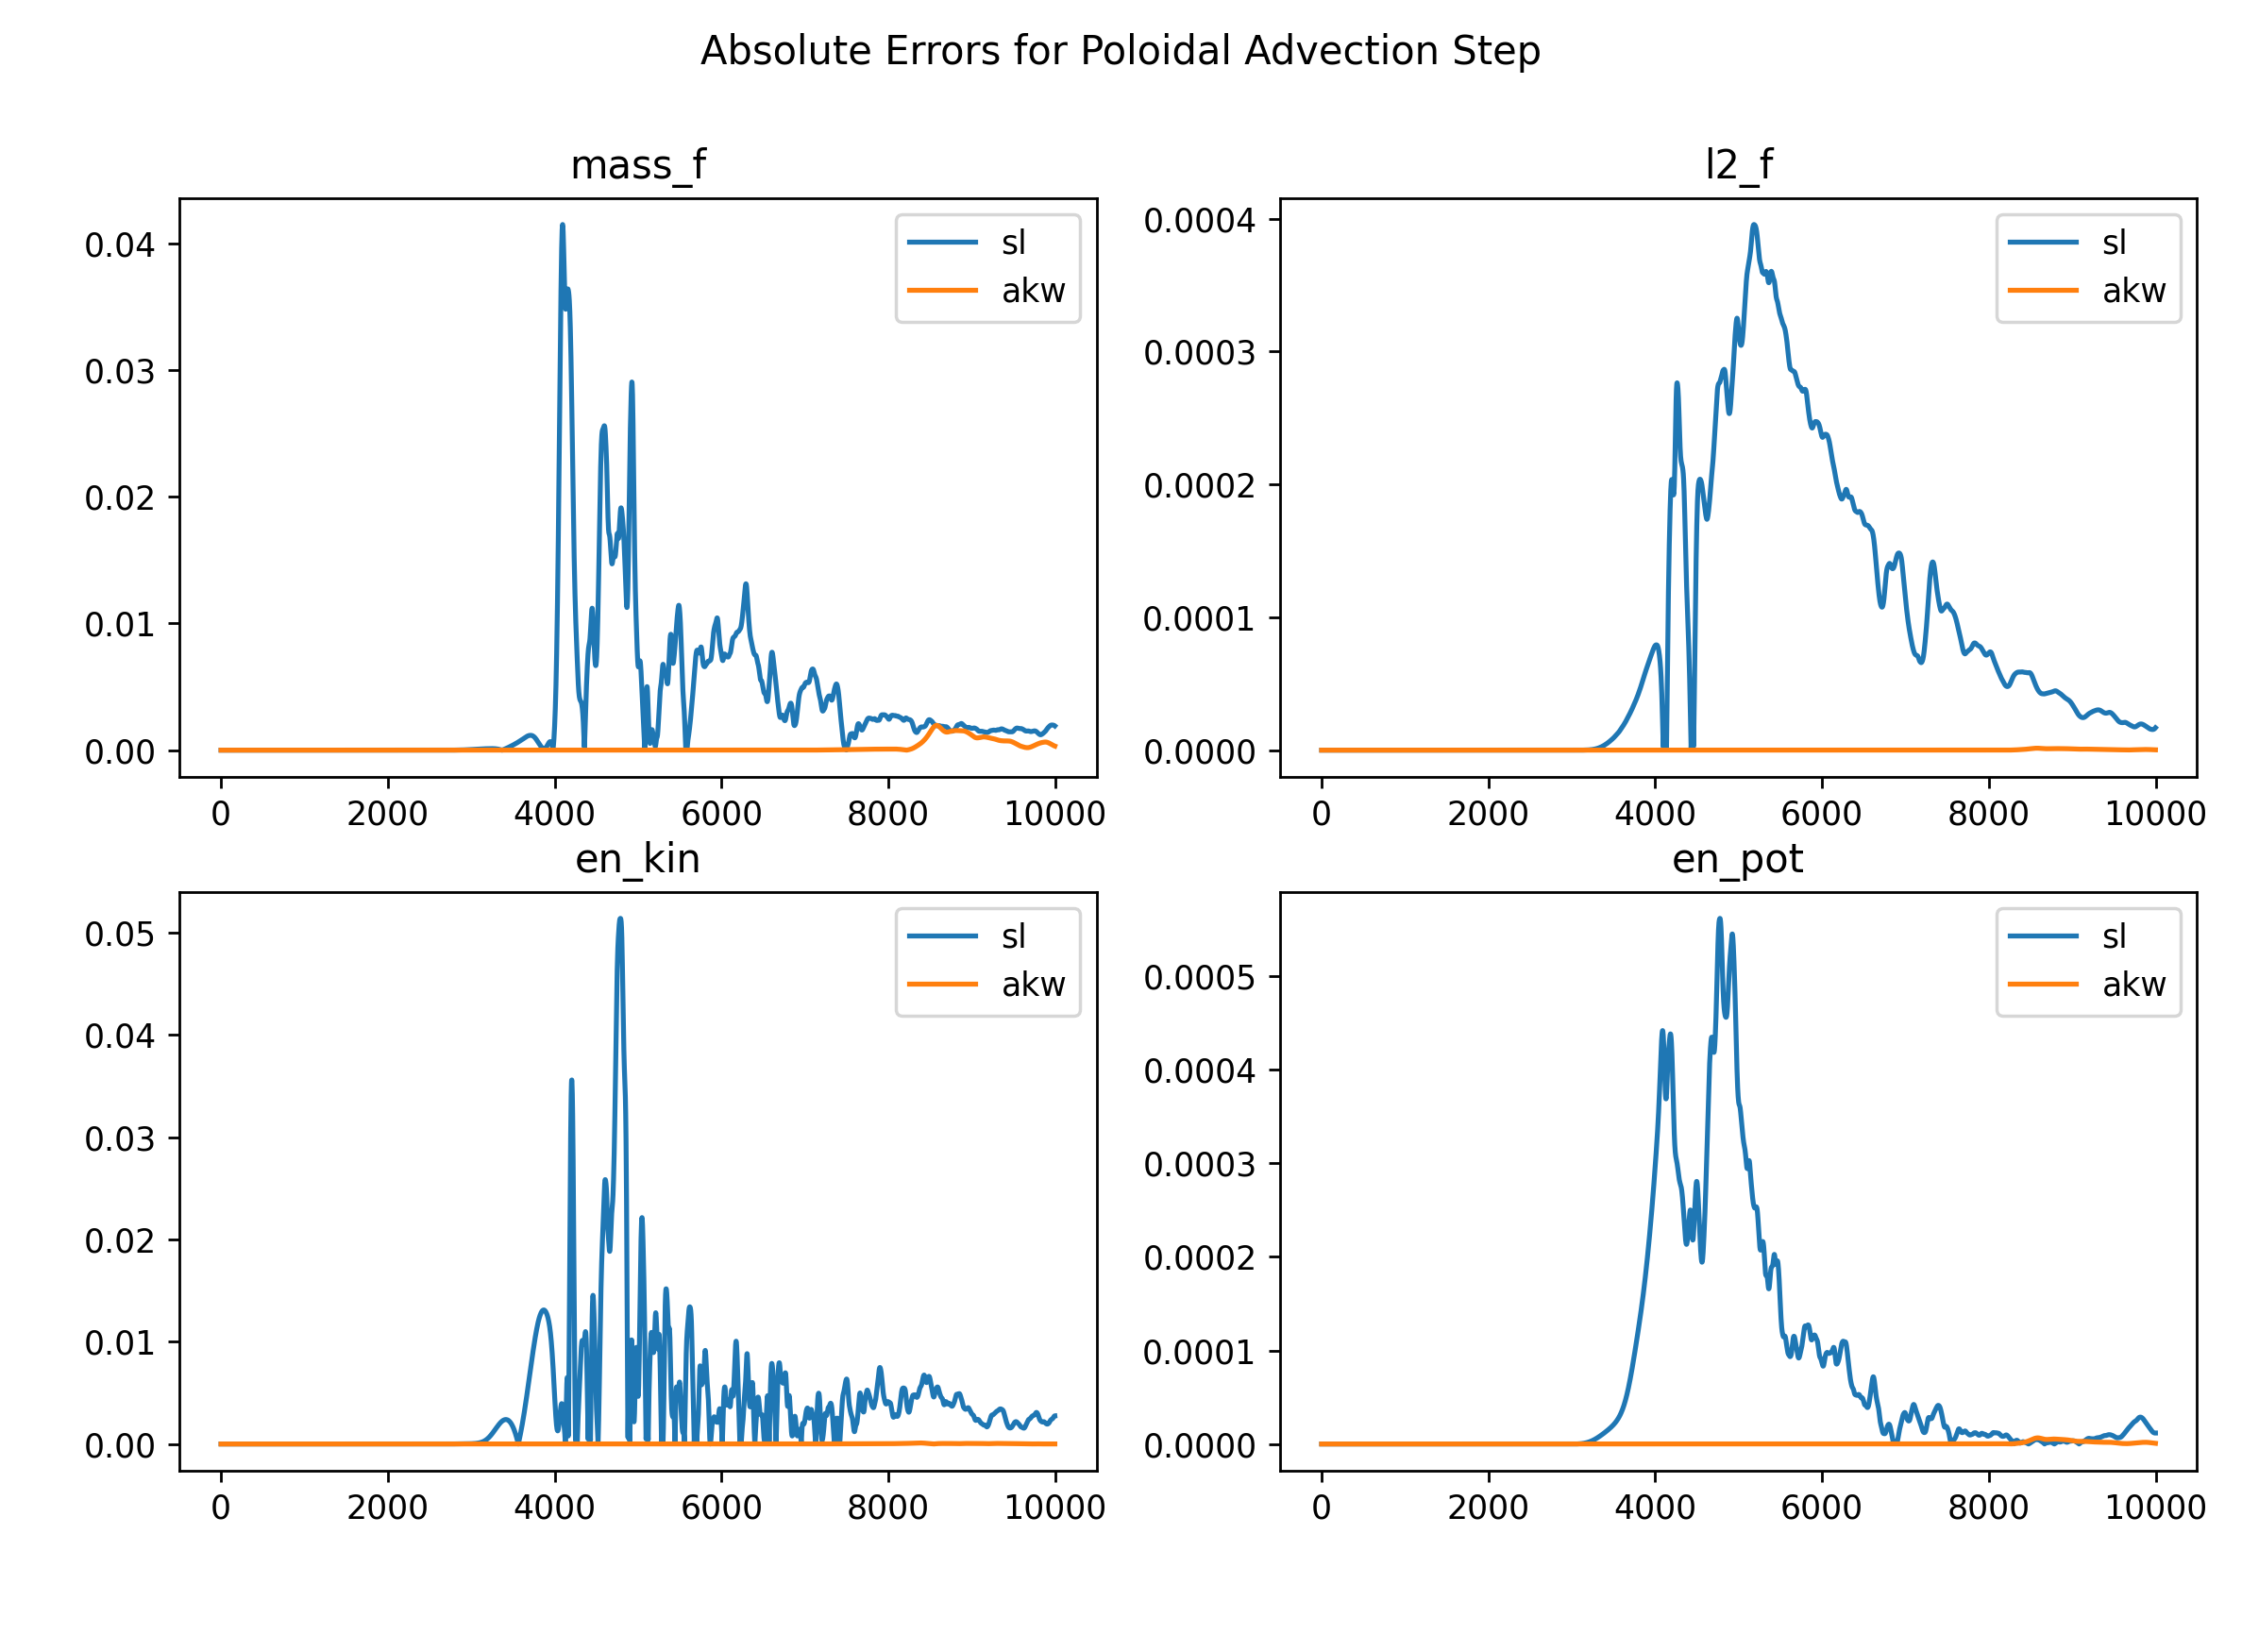
\includegraphics[width=0.9\linewidth]{abs_err dt2}
	\caption{The absolute error for different quantities before and after the poloidal advection step with time step-size $\Delta t = 2$.}
	\label{fig:abserr_dt2}
\end{figure}


\begin{figure}
	\centering
	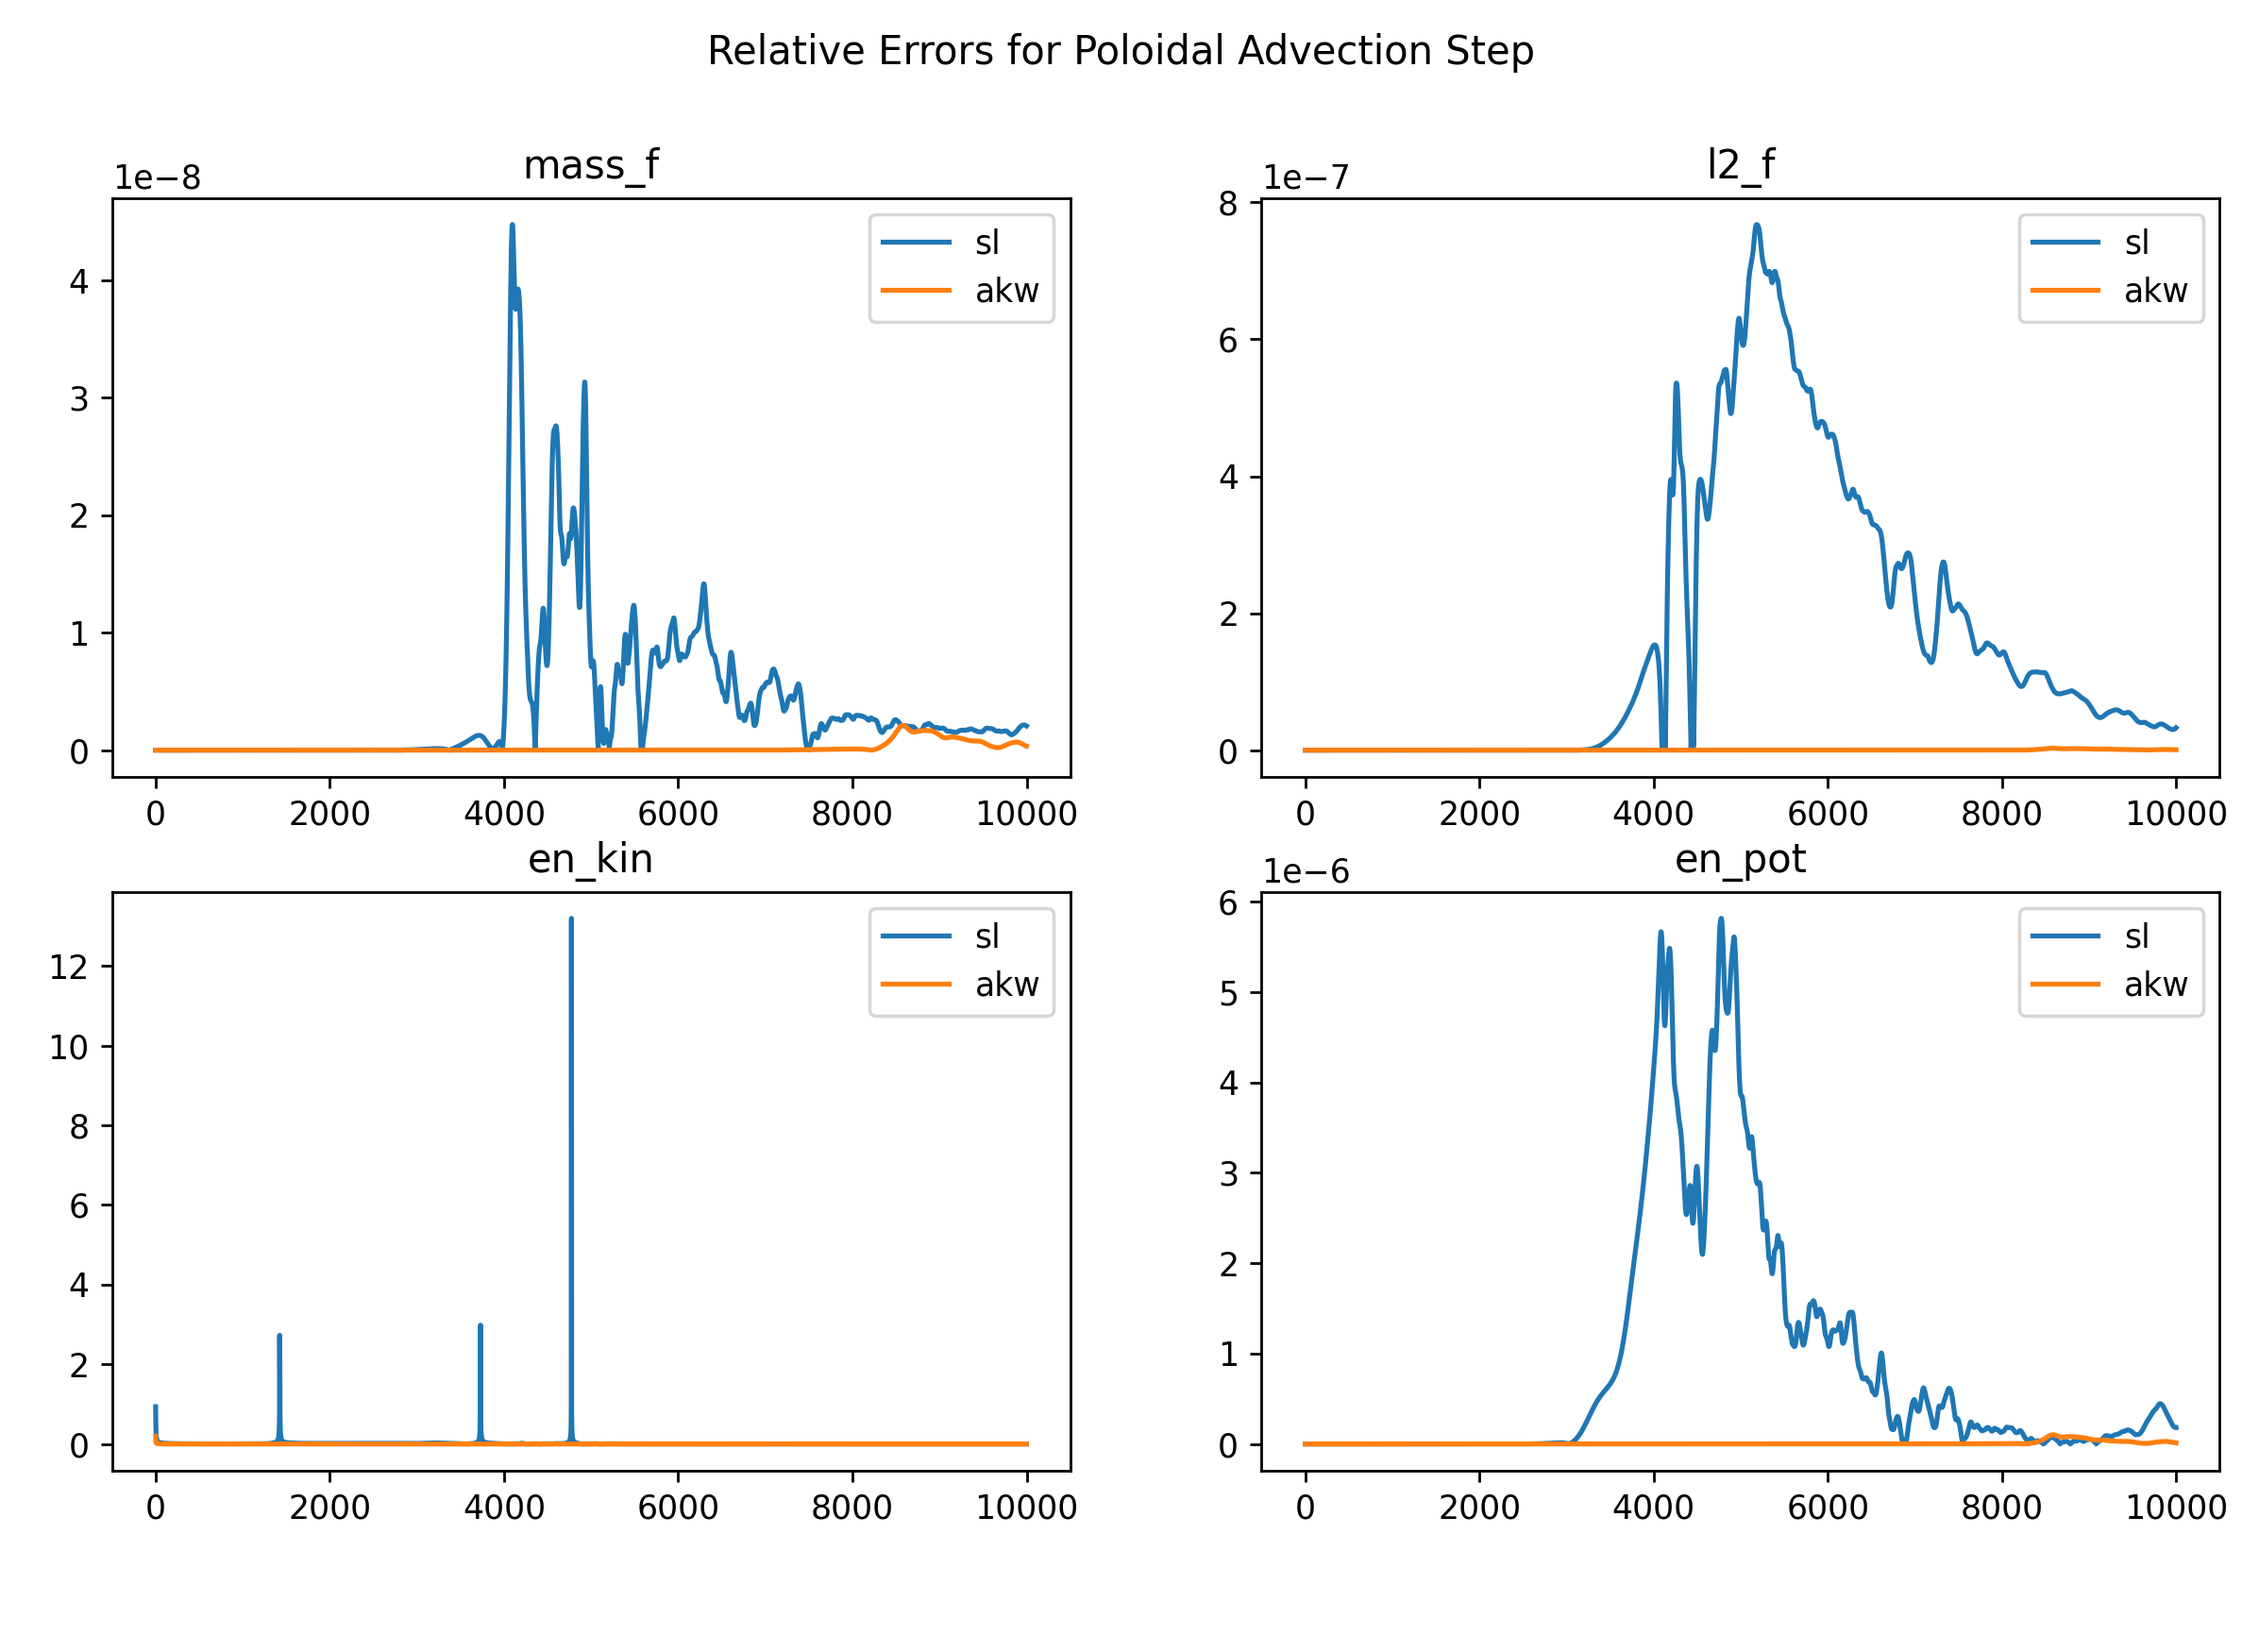
\includegraphics[width=0.9\linewidth]{rel_err dt2}
	\caption{The relative error for different quantities before and after the poloidal advection step with time step-size $\Delta t = 2$.}
	\label{fig:relerr_dt2}
\end{figure}


\begin{figure}
	\centering
	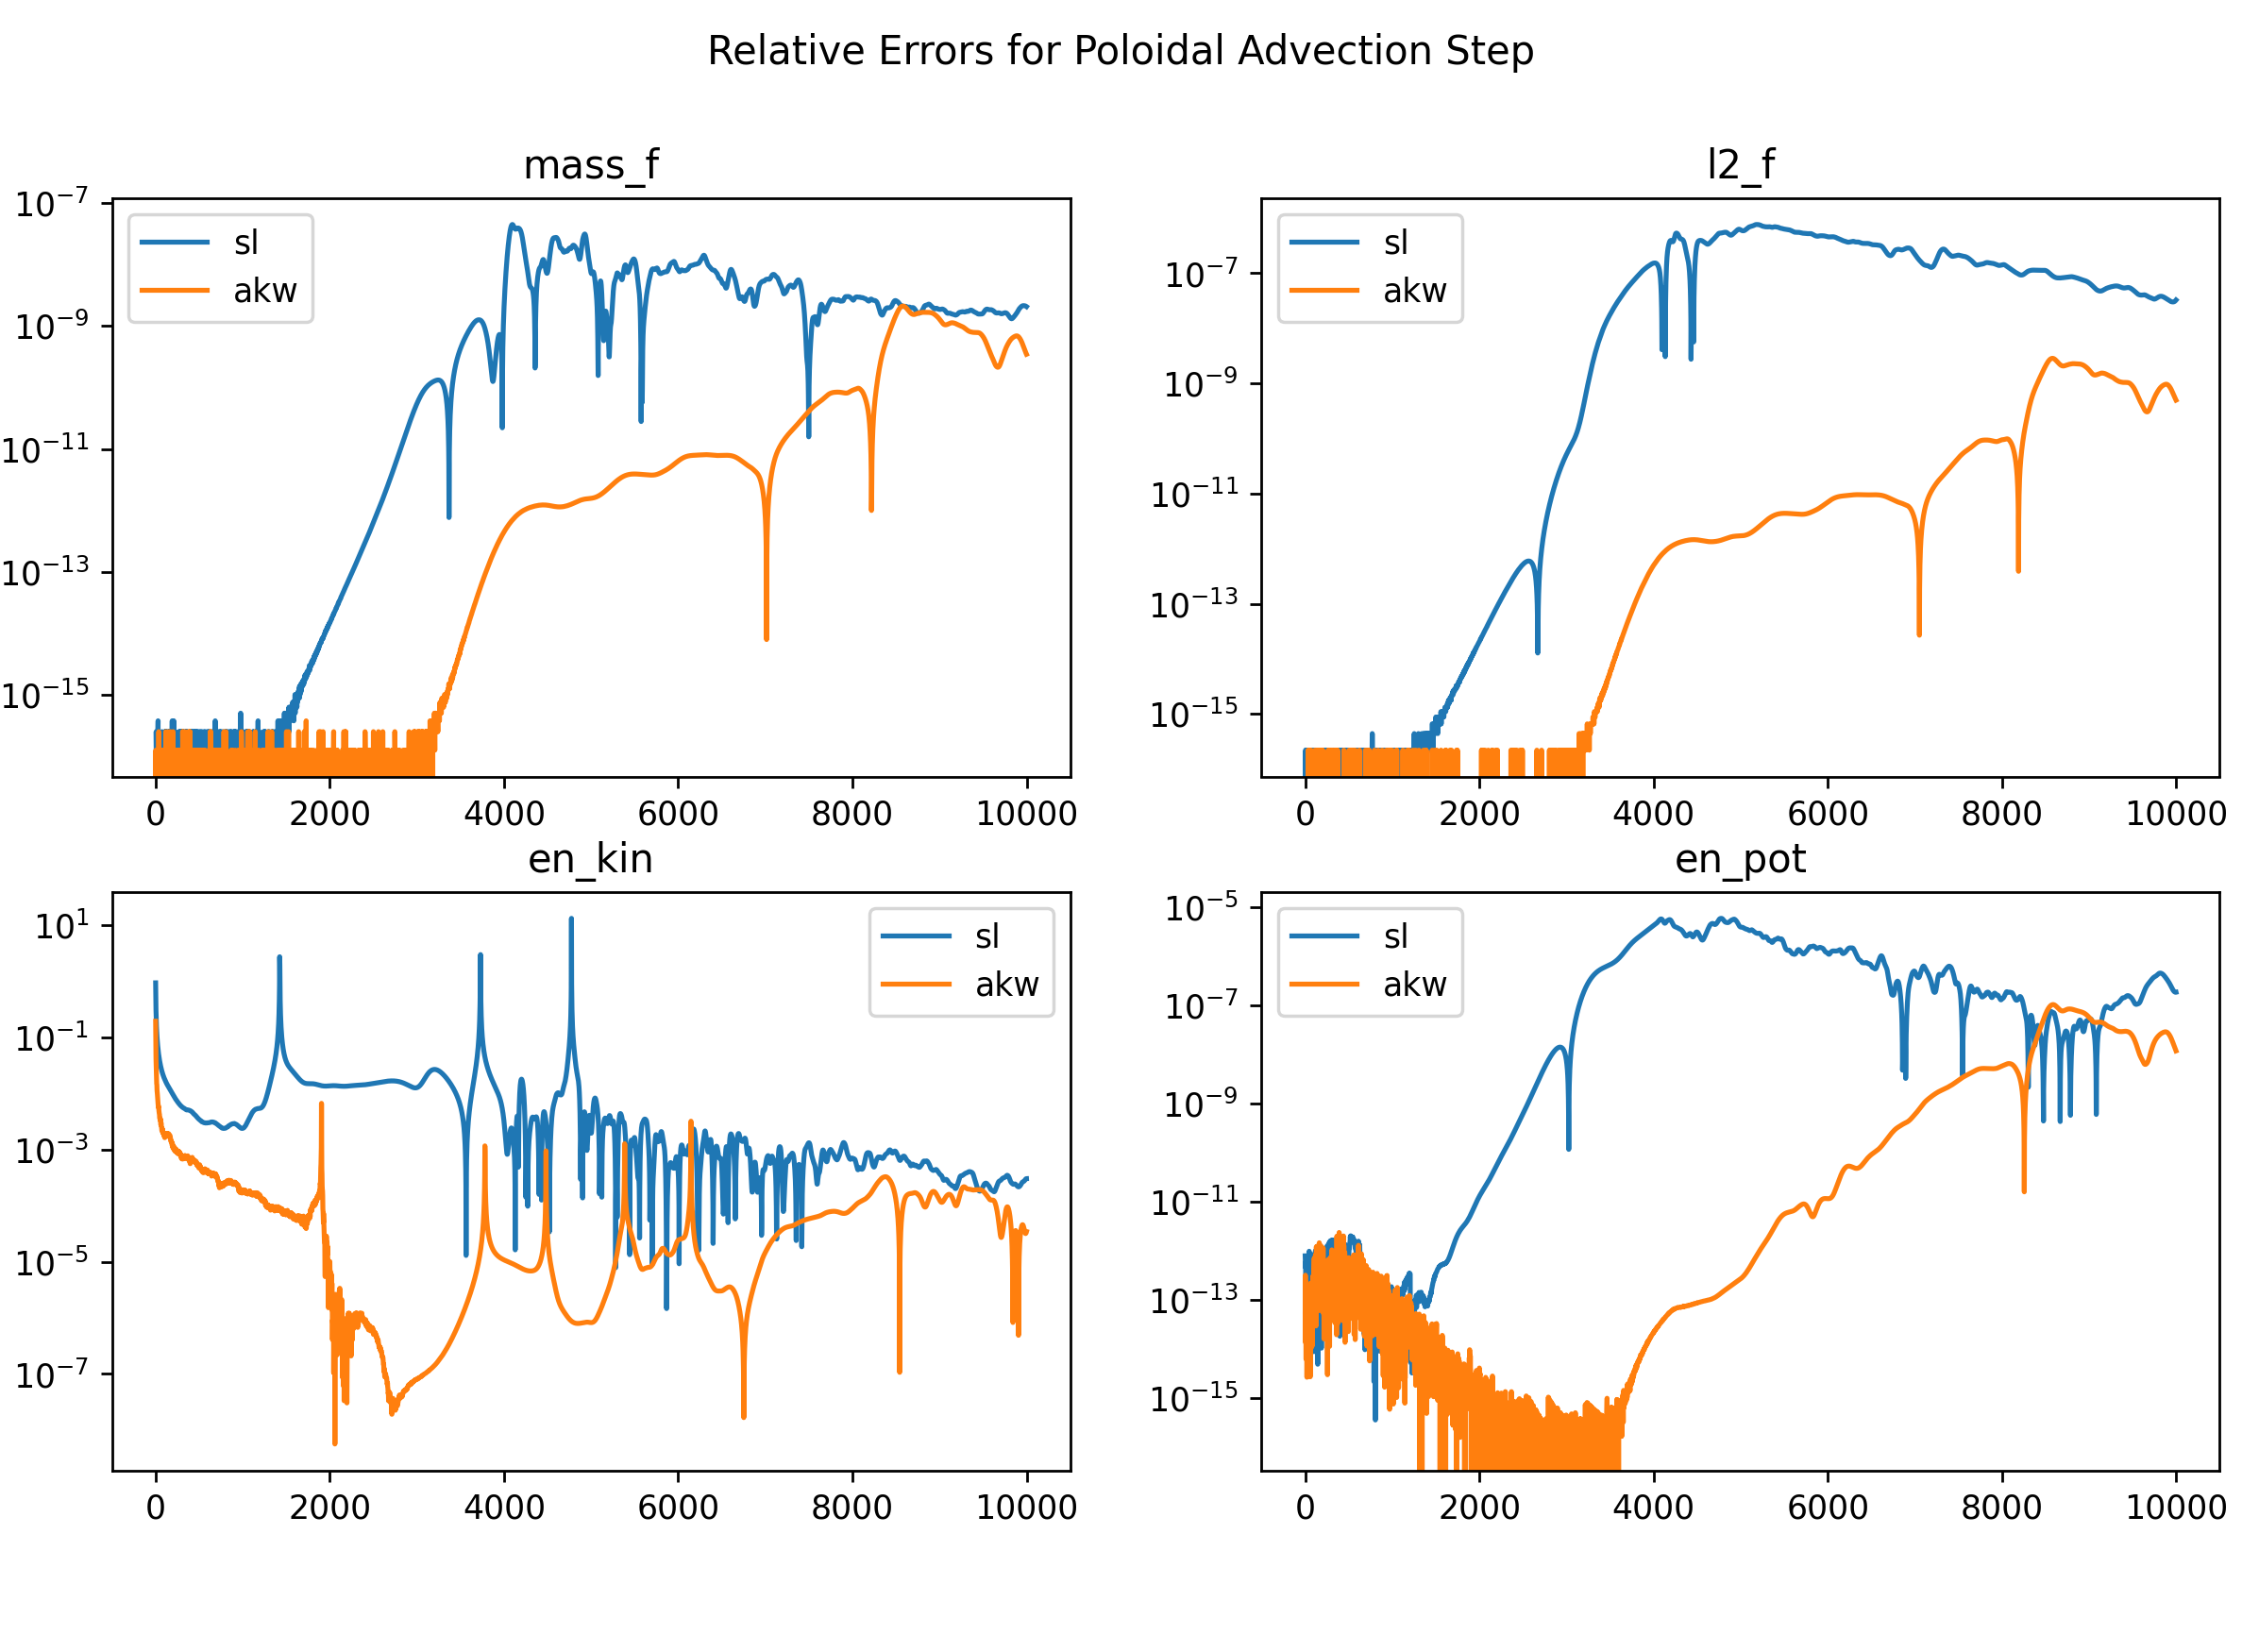
\includegraphics[width=0.9\linewidth]{rel_err_log dt2}
	\caption{The relative error for different quantities before and after the poloidal advection step on a semi-logarithmic scale with time step-size $\Delta t = 2$.}
	\label{fig:relerrlog_dt2}
\end{figure}


\begin{figure}
	\centering
	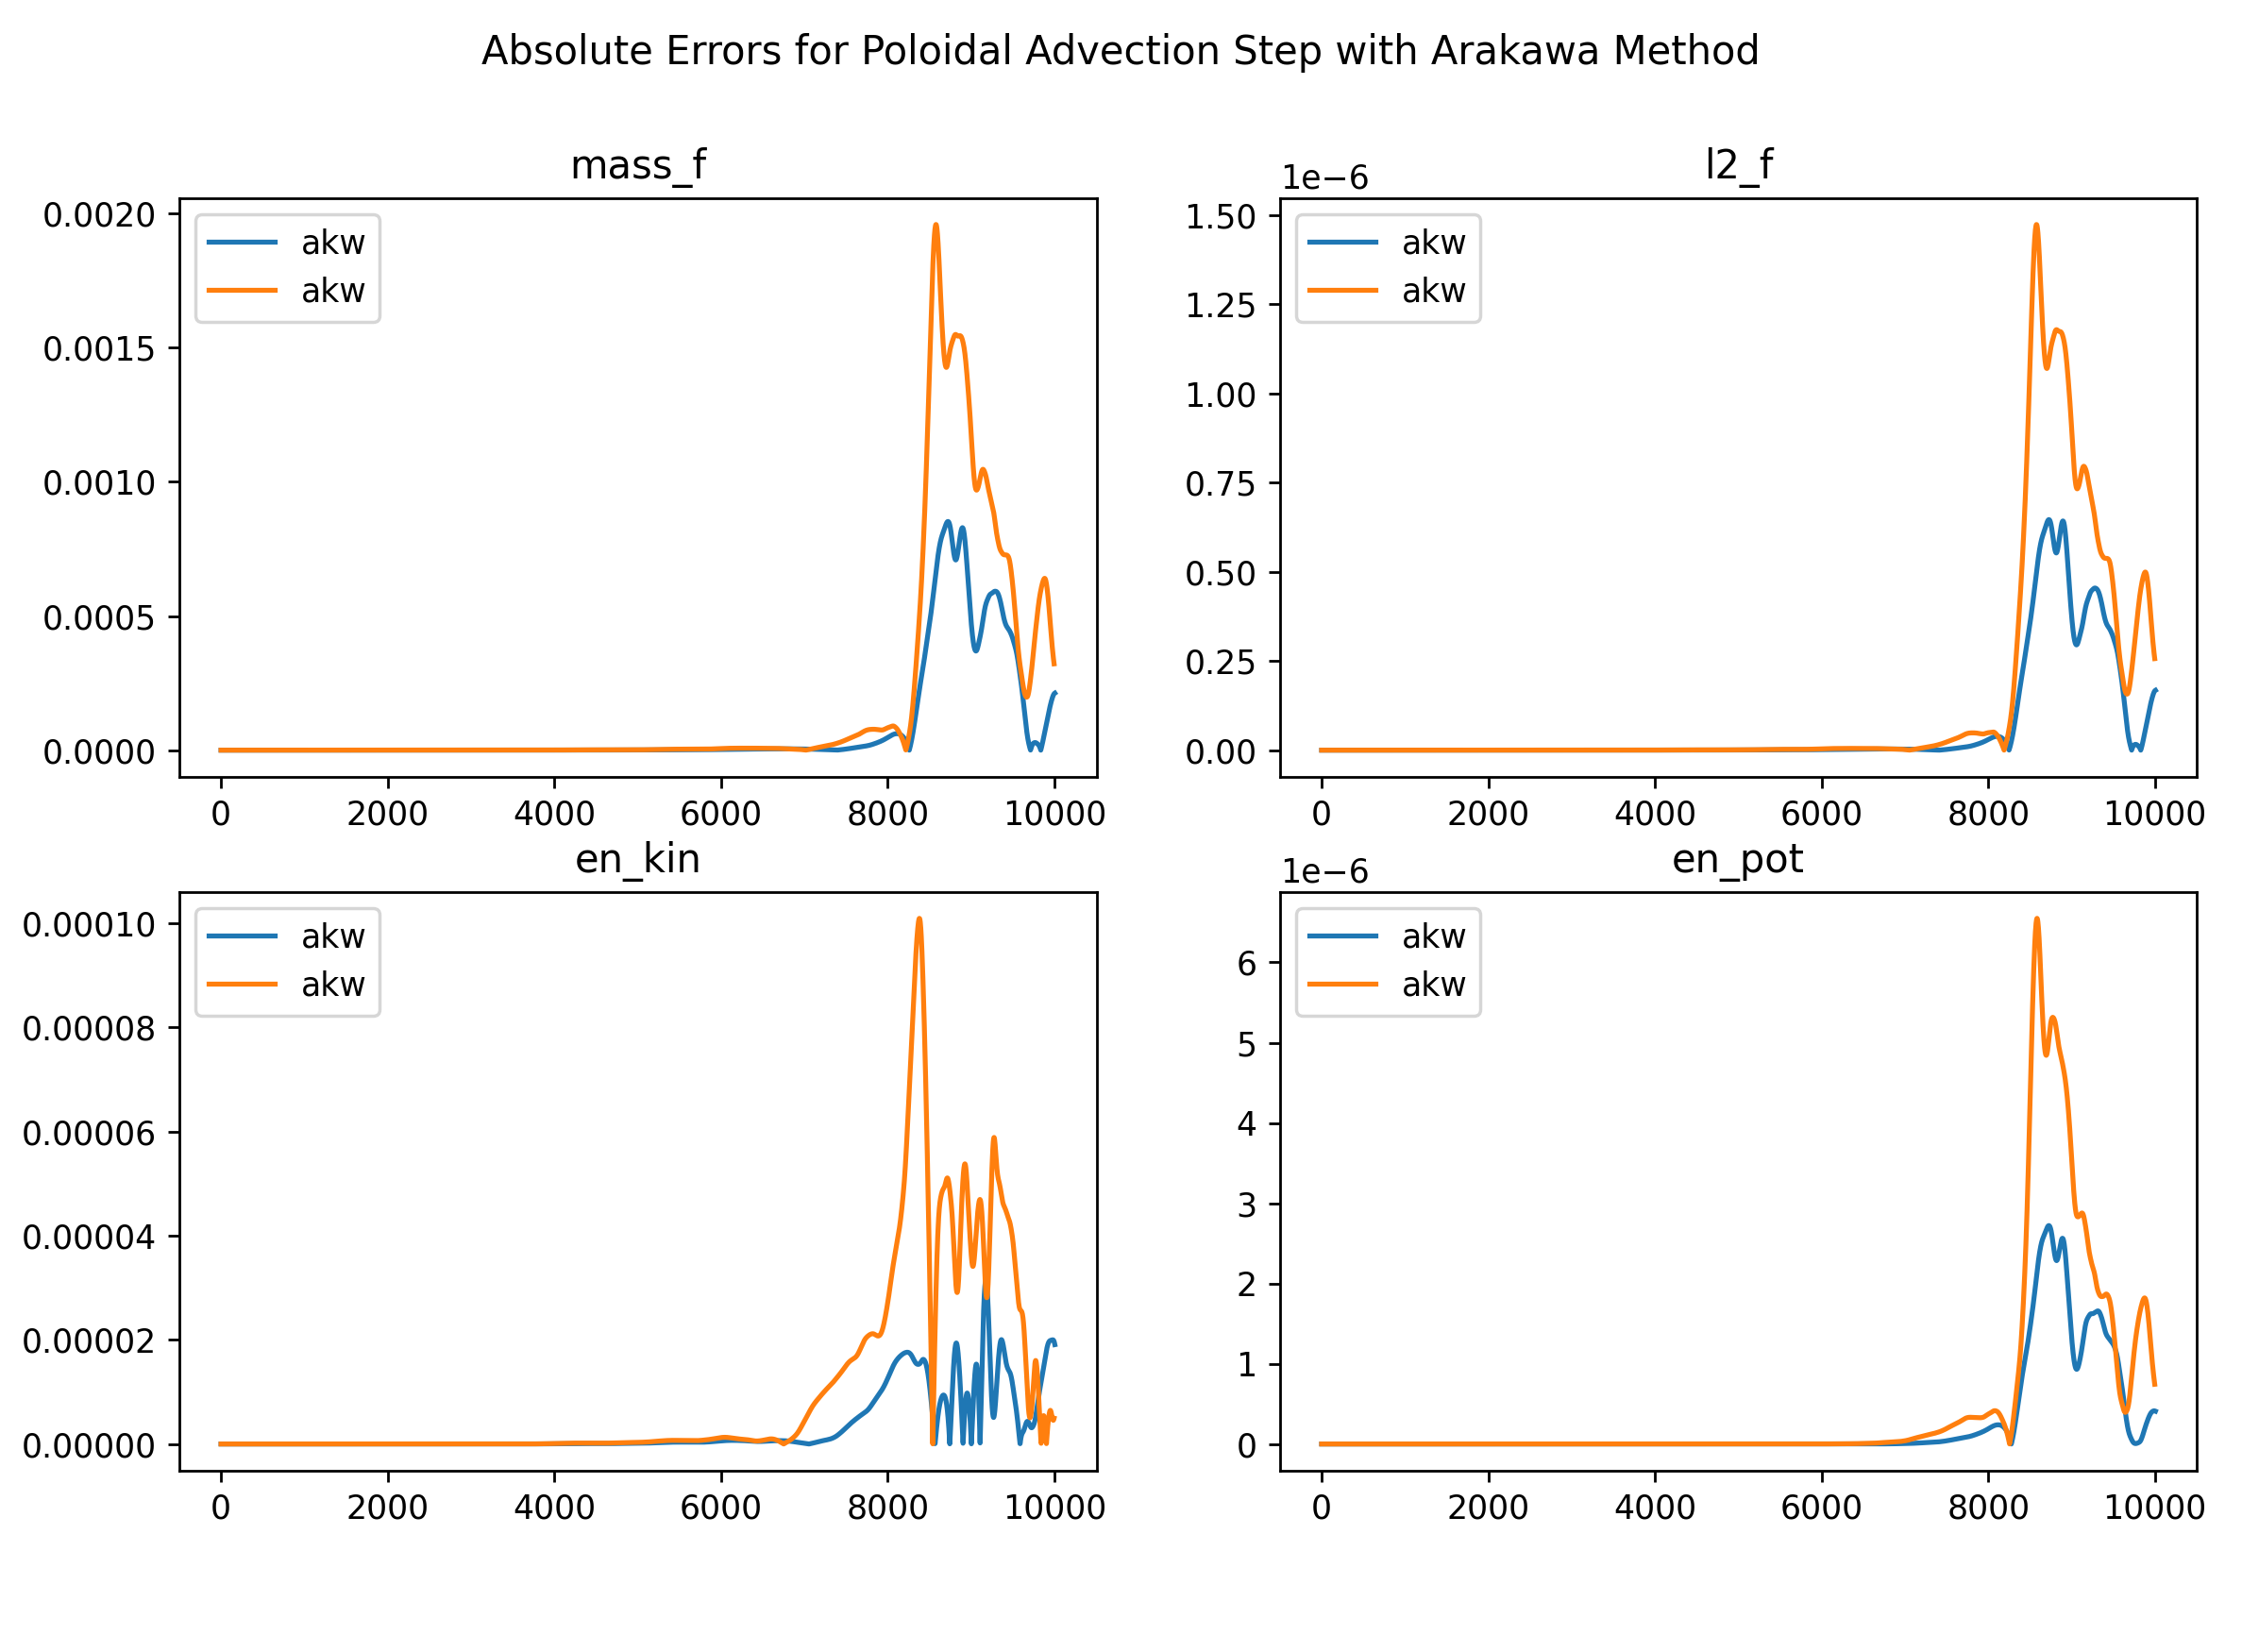
\includegraphics[width=0.9\linewidth]{abs_err akw}
	\caption{The absolute error for different quantities before and after the poloidal advection step with the Arakawa method, comparing time step-size $\Delta t = 1$ and $\Delta t = 2$.}
	\label{fig:abserr_akw}
\end{figure}


\begin{figure}
	\centering
	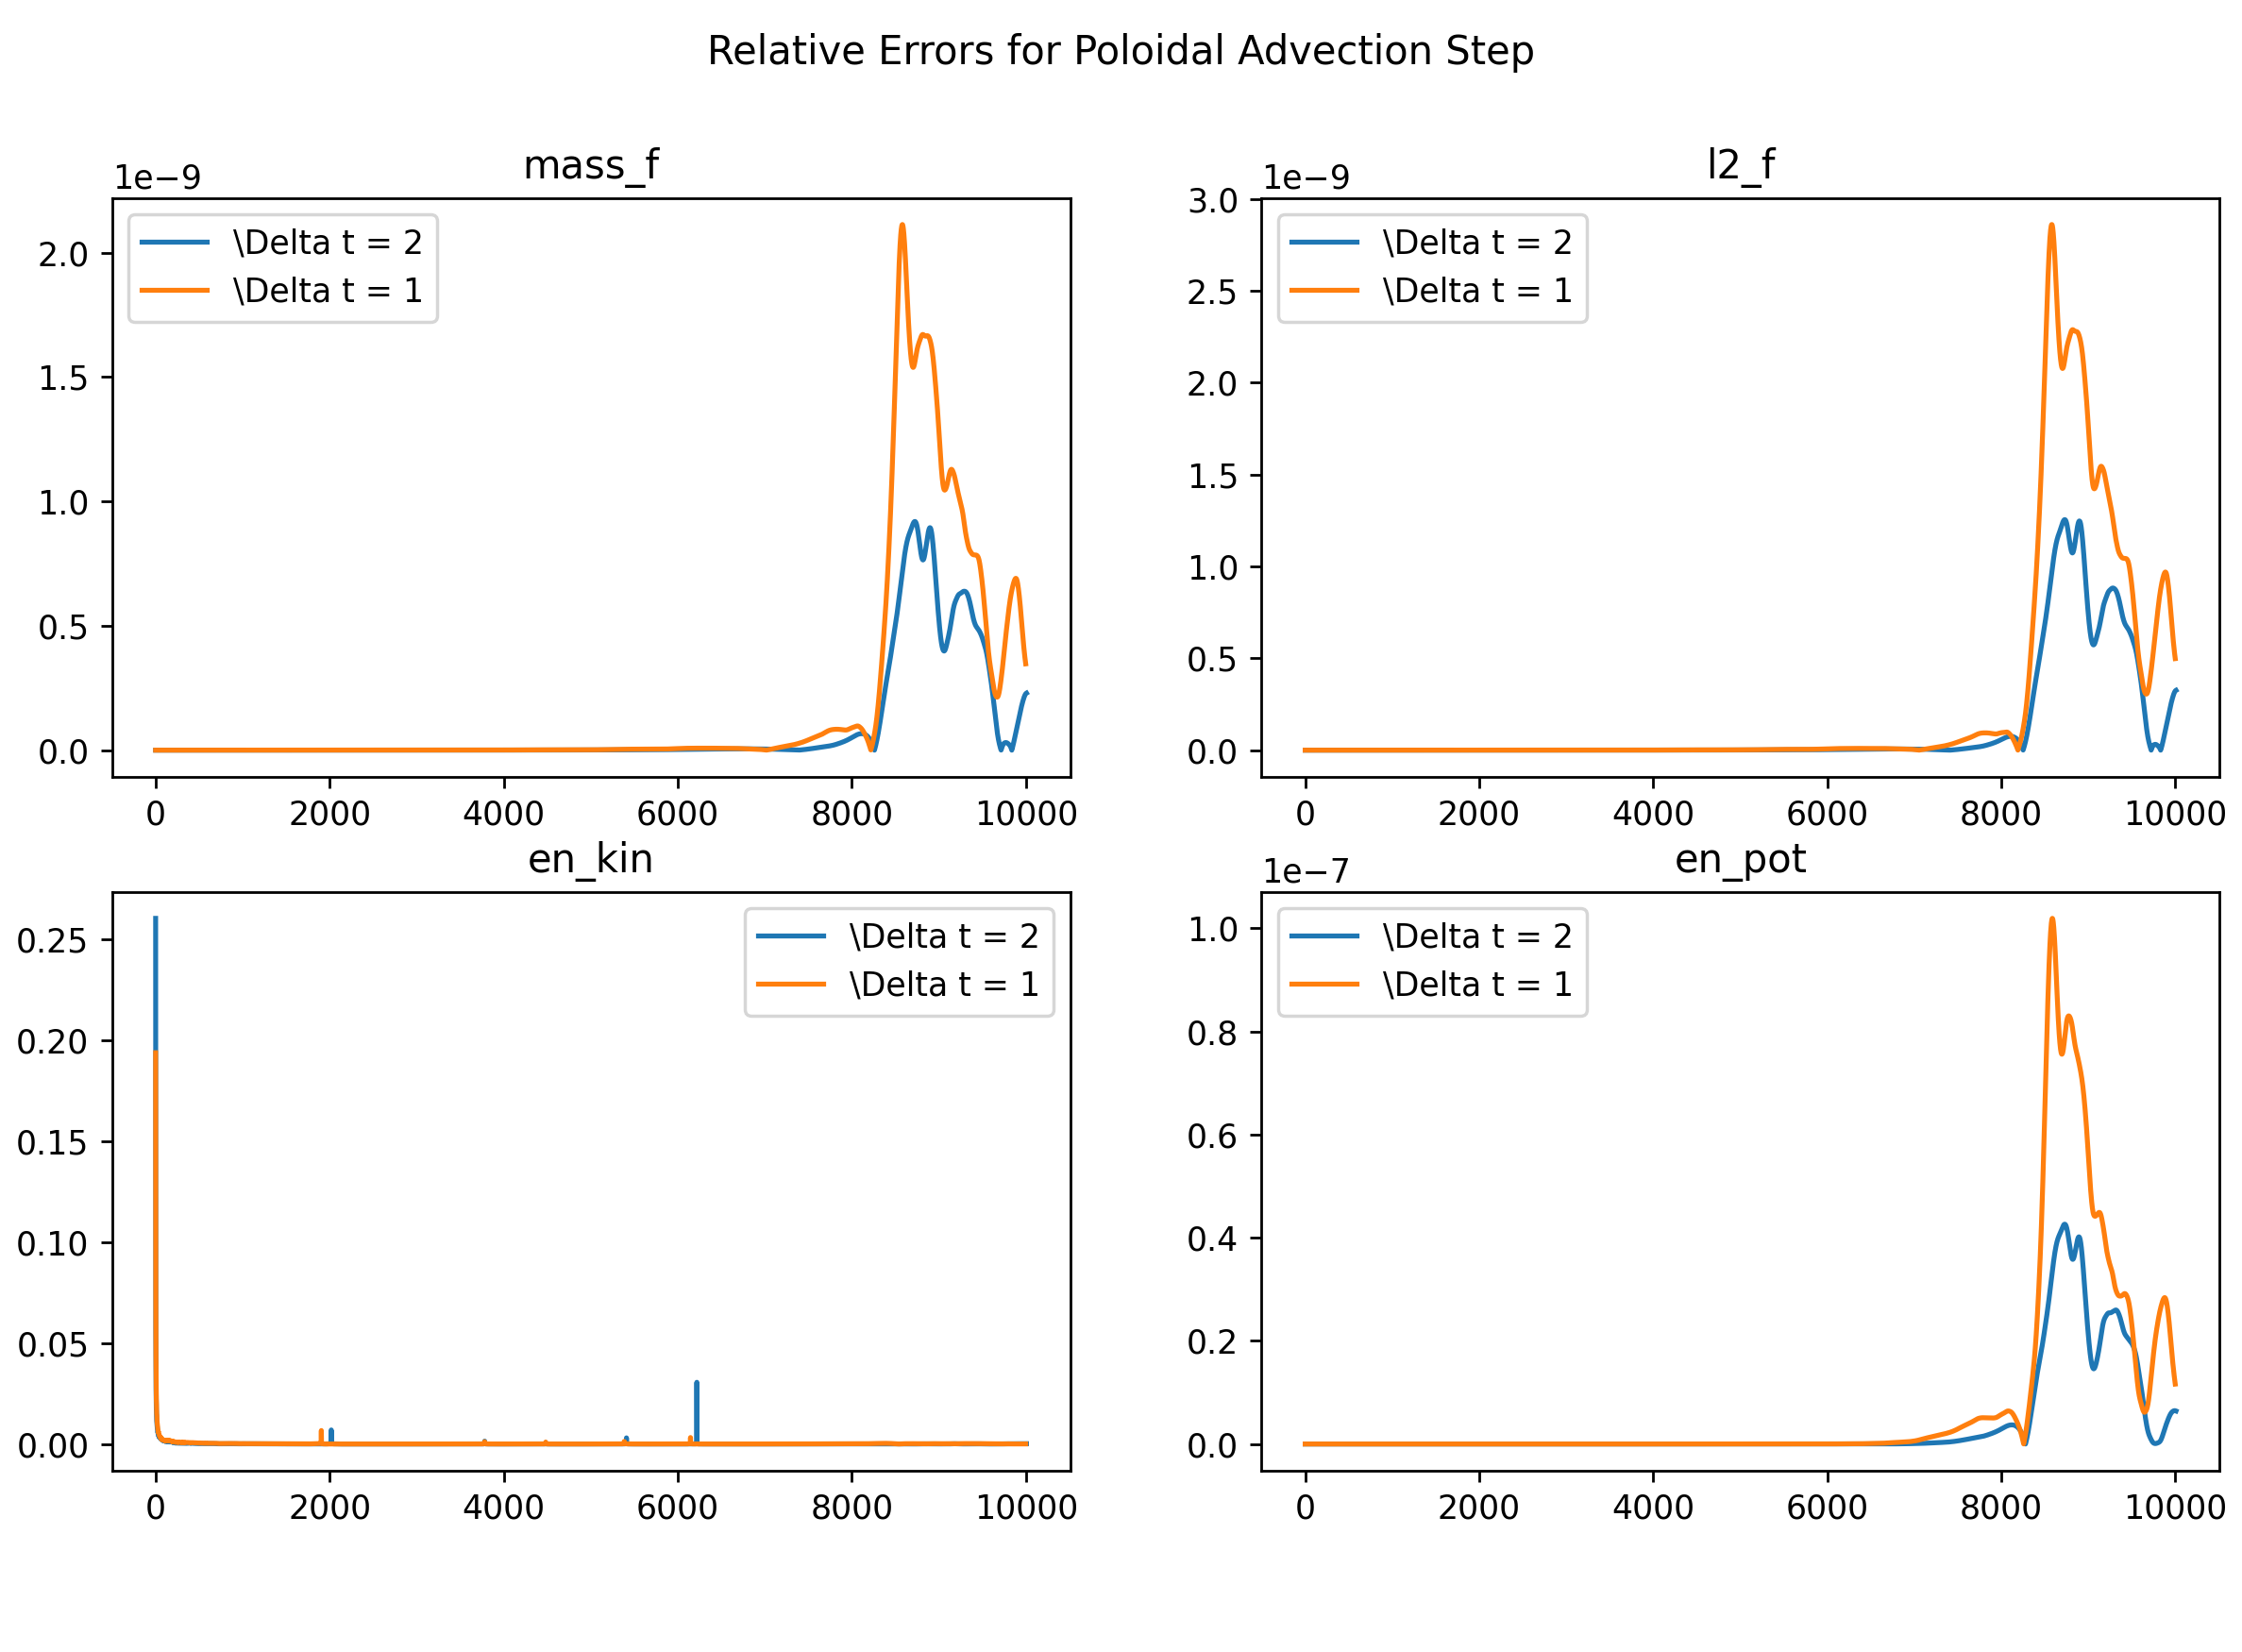
\includegraphics[width=0.9\linewidth]{rel_err akw}
	\caption{The relative error for different quantities before and after the poloidal advection step with the Arakawa method, comparing time step-size $\Delta t = 1$ and $\Delta t = 2$..}
	\label{fig:relerr_akw}
\end{figure}


\begin{figure}
	\centering
	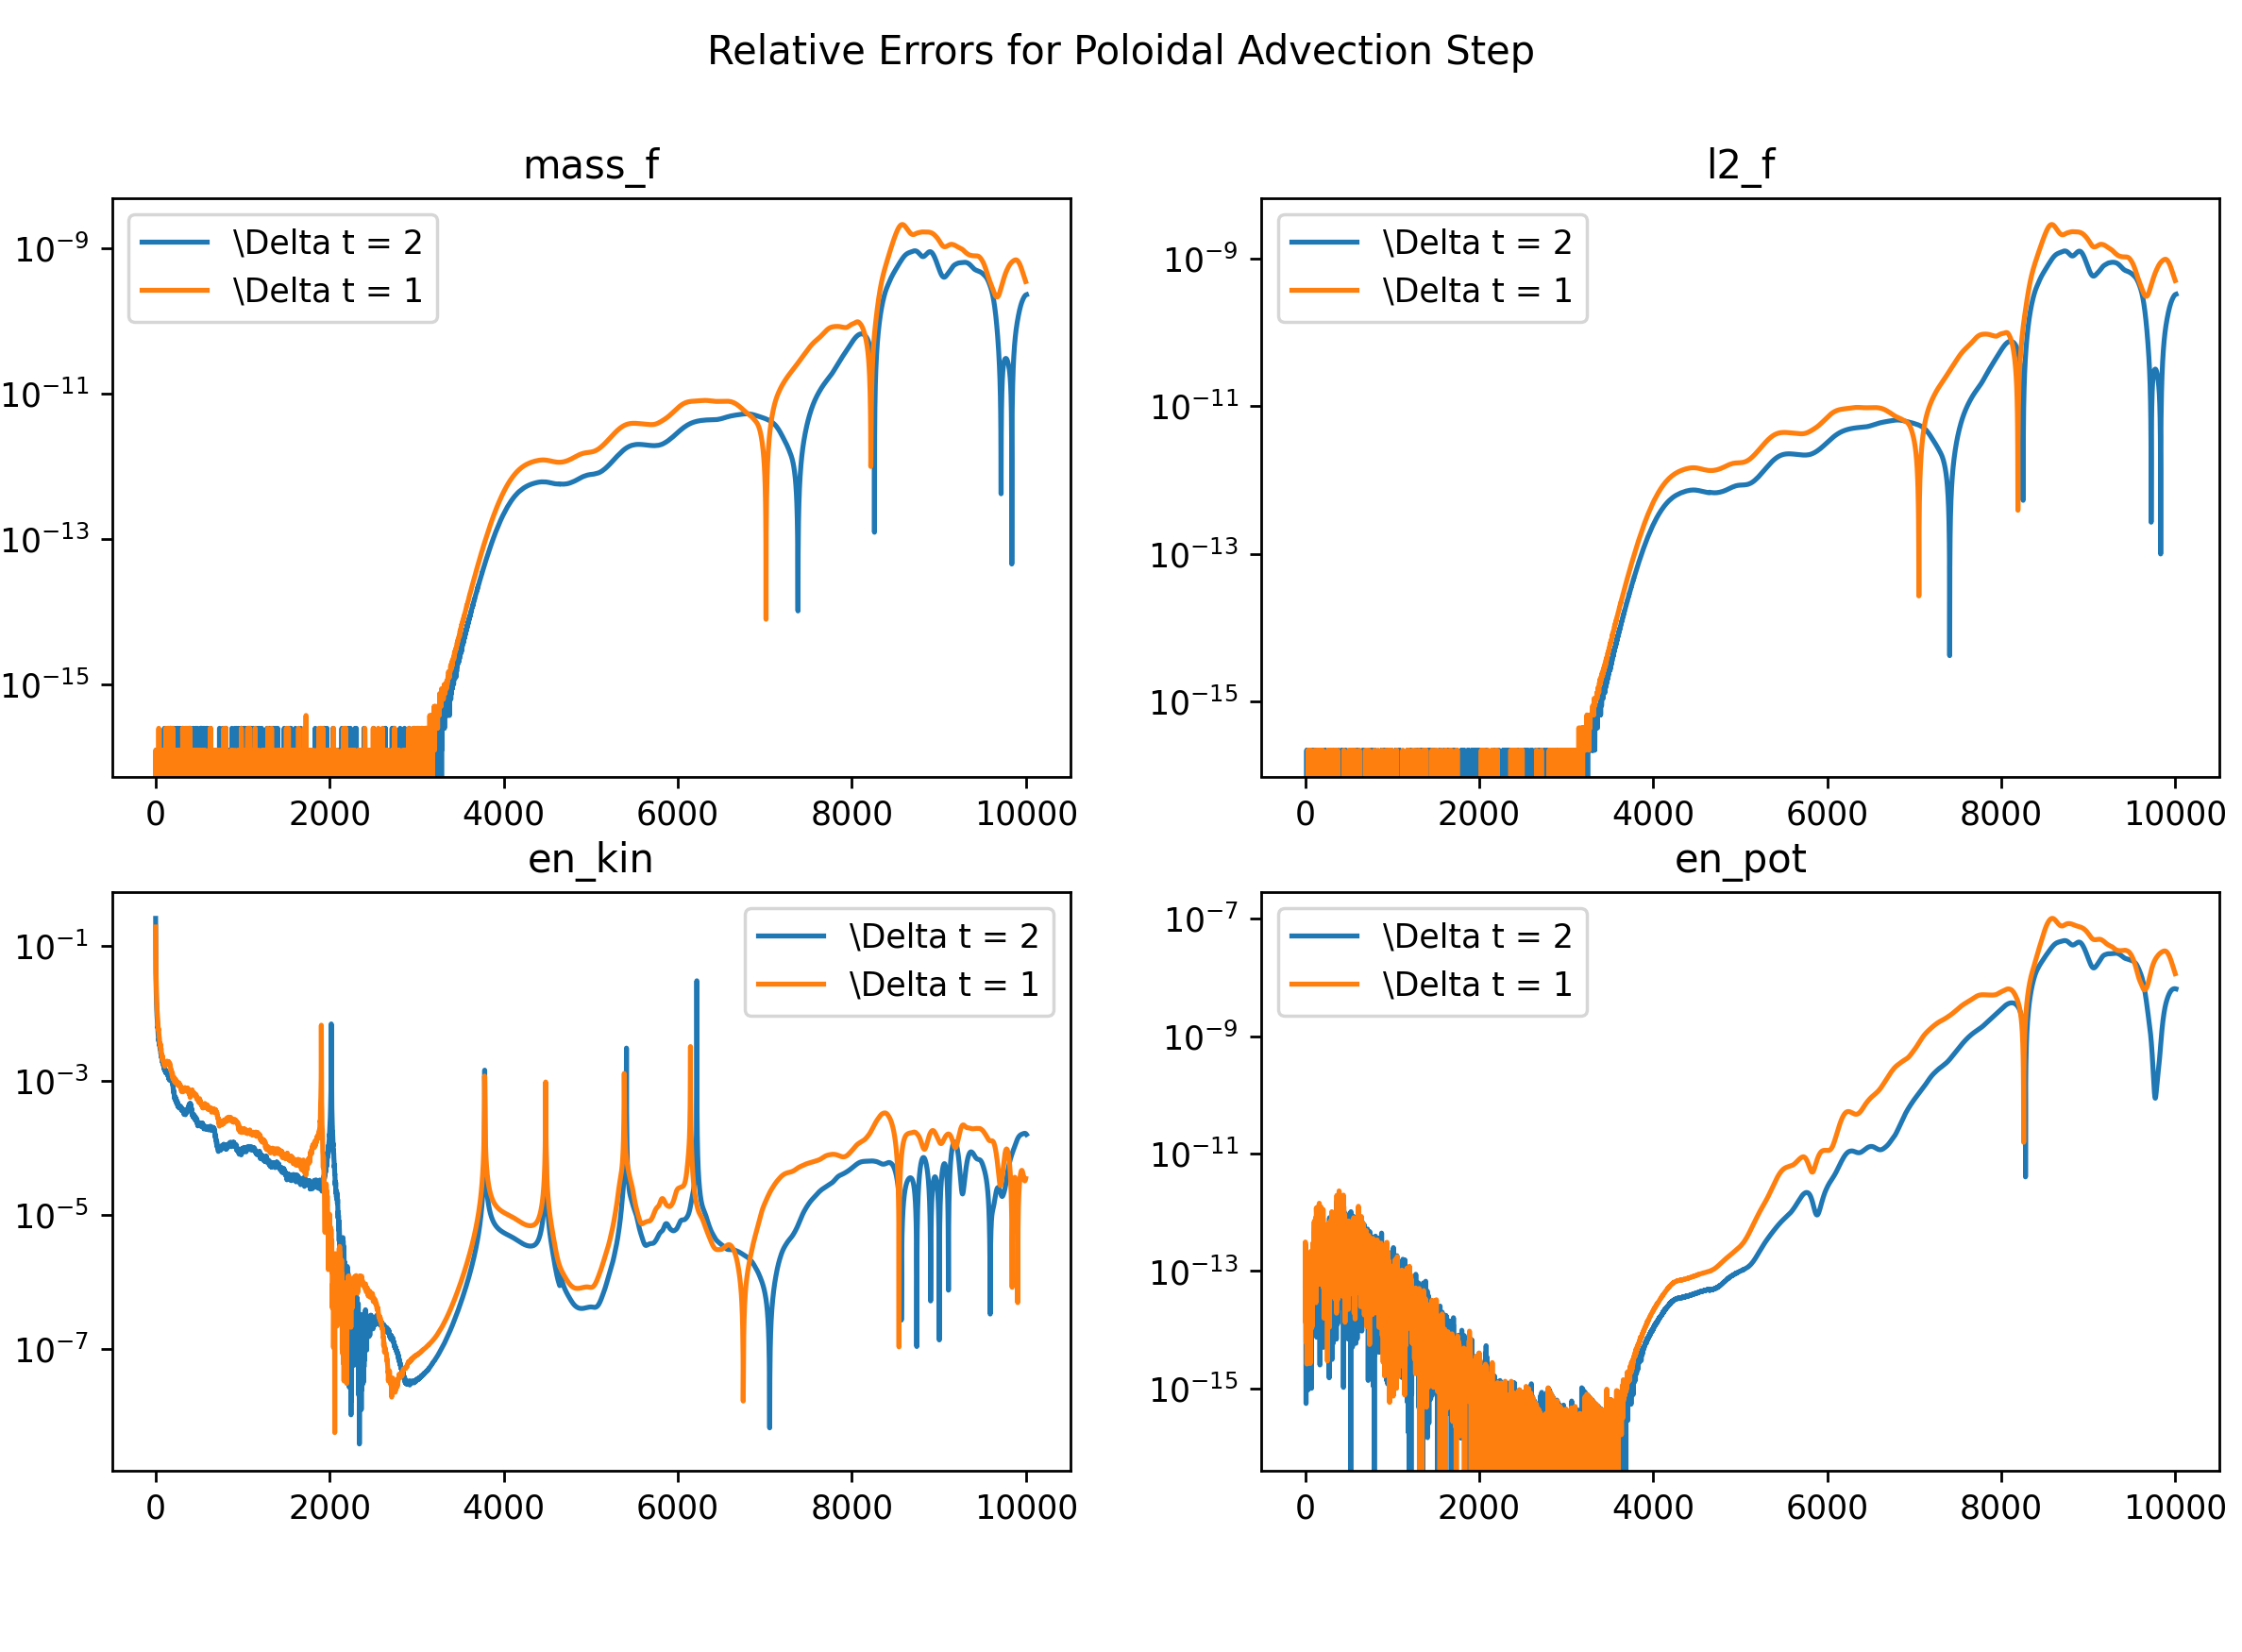
\includegraphics[width=0.9\linewidth]{rel_err_log akw}
	\caption{The relative error for different quantities before and after the poloidal advection step on a semi-logarithmic scale with the Arakawa method, comparing time step-size $\Delta t = 1$ and $\Delta t = 2$..}
	\label{fig:relerrlog_akw}
\end{figure}



